\documentclass{rubeamer}
\svnid{$Id: FinalPresentation.tex 2719 2015-11-05 12:57:01Z kristofert13 $}
\svnidlong{$HeadURL: https://repository.cs.ru.is/svn/t-411-mech-2015/group/TiltIt/FinalPresentation/FinalPresentation.tex $}
{$LastChangedDate: 2015-11-05 12:57:01 +0000 (fim., 05 nóv. 2015) $}
{$LastChangedRevision: 2719 $}
{$LastChangedBy: kristofert13 $}
% if you'd like the above information to be updated,
% use svn properties to set svn:keywords to for Id and URL (or HeadURL)
% Don't forget to set the draft to final before 
\addbibresource{references.bib}
\usepackage{hyperref}


\begin{document}
%----------- titlepage ----------------------------------------------%
\rutitleframe{}

%----------- slides ----------------------------------------------%

\begin{frame}{Rannsóknarefni}
	\begin{itemize}
		\item Dreifing sólmyrkva á jörðinni
		\item Dreifing átaka á jörðinni
		\item Er fylgni milli sólmyrkva og stríðsátaka
		
	\end{itemize}
	\note{Kynna sp. og útgangspunk rannsóknar }
\end{frame}

\begin{frame}{Gagnasafnið}
	\vspace{2em}
	\begin{itemize}
		\item Átök - Háskólinn í Uppsölum, Svíþjóð \cite{conflict}
		\item Sólmyrkvar - NASA \cite{Eclipse}
		\item Vopnasala - Stockholm intern. peace research institution \cite{weapon}
	\end{itemize}
	\note{Hvaðan koma gögnin + hvað þurfti að gera við gögnin til að gera þau nýtileg }
	
	\begin{figure}
		\centering
		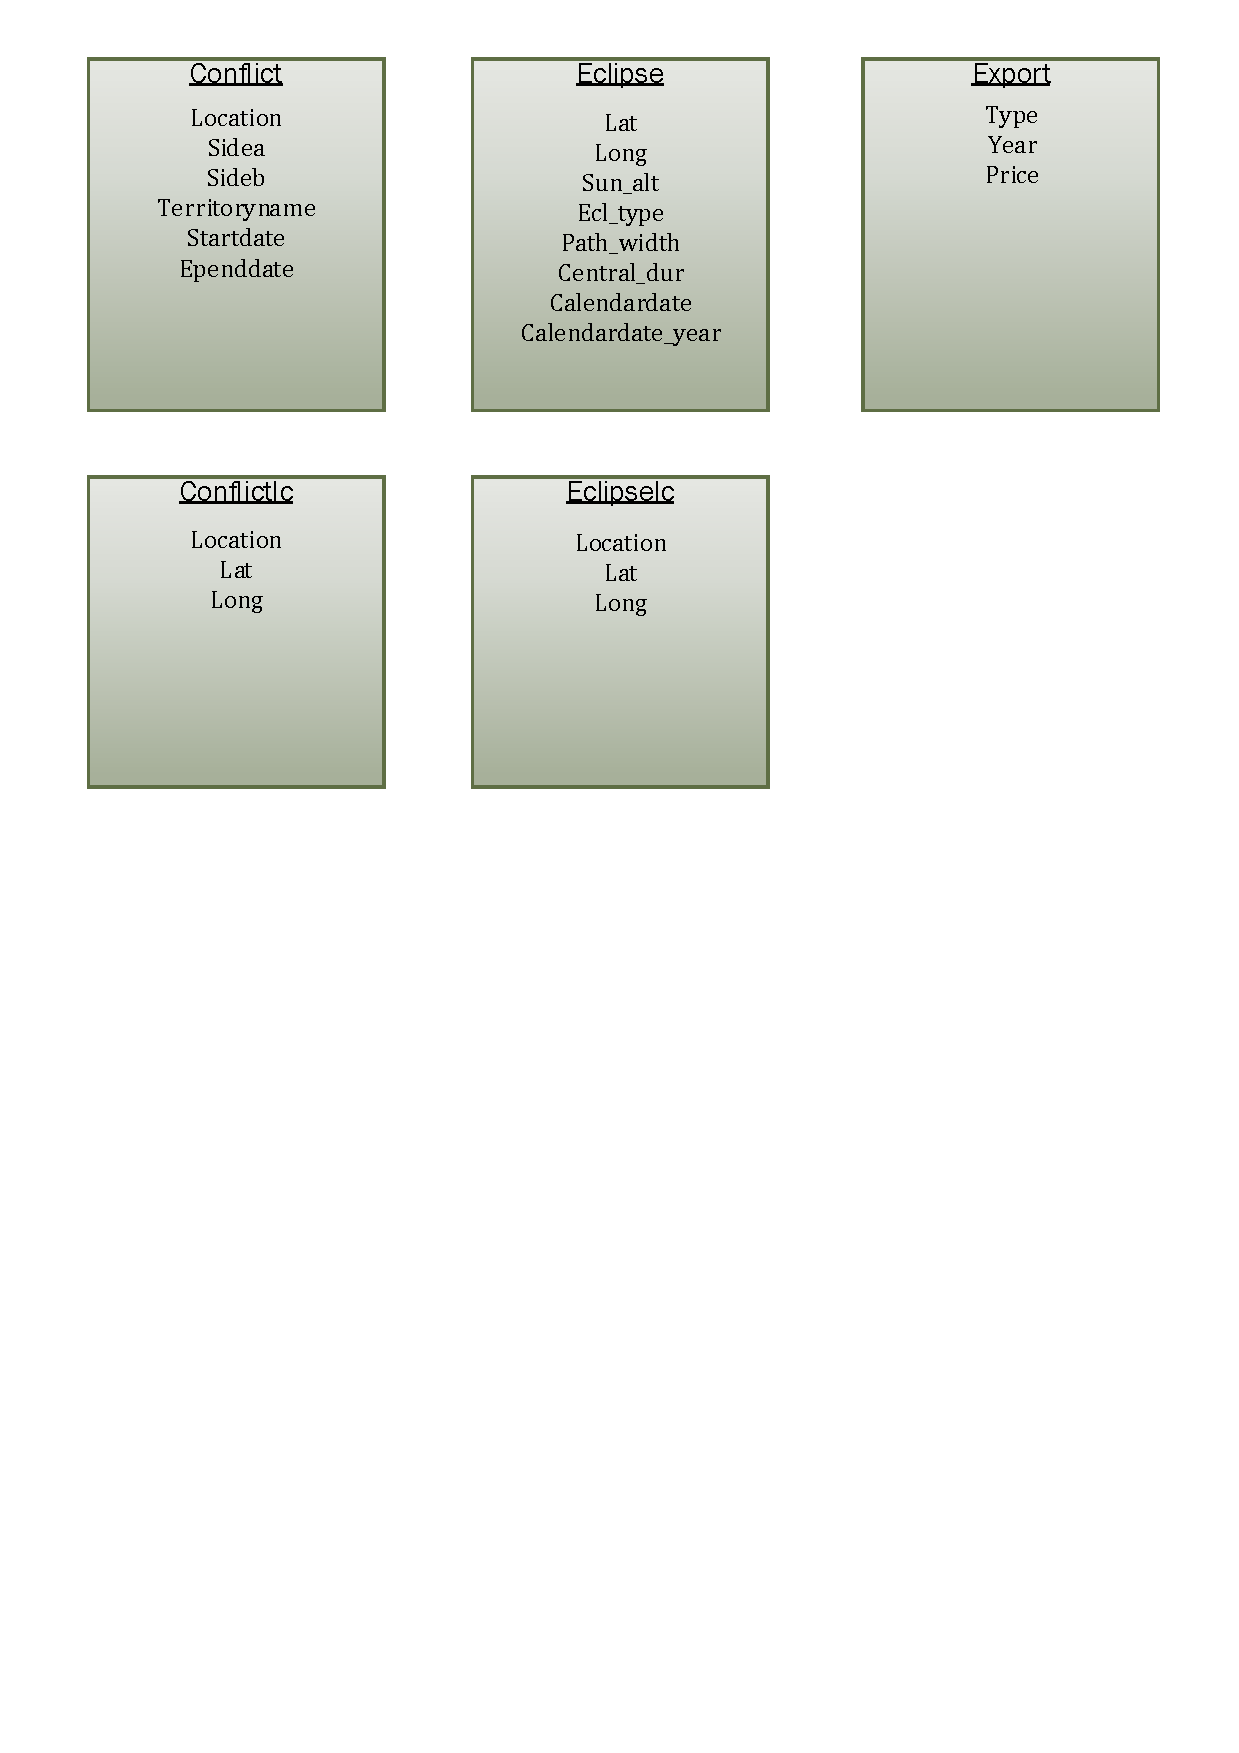
\includegraphics[width = 8cm]{dataSchemaKynn.pdf}
	\end{figure}
\end{frame}

\begin{frame}{GUI}
	\begin{itemize}
		\item GUI unnið í PyQt4 \cite{qt4}, hannað í Qt4-Designer
	\end{itemize}
	\begin{figure}
		\centering
		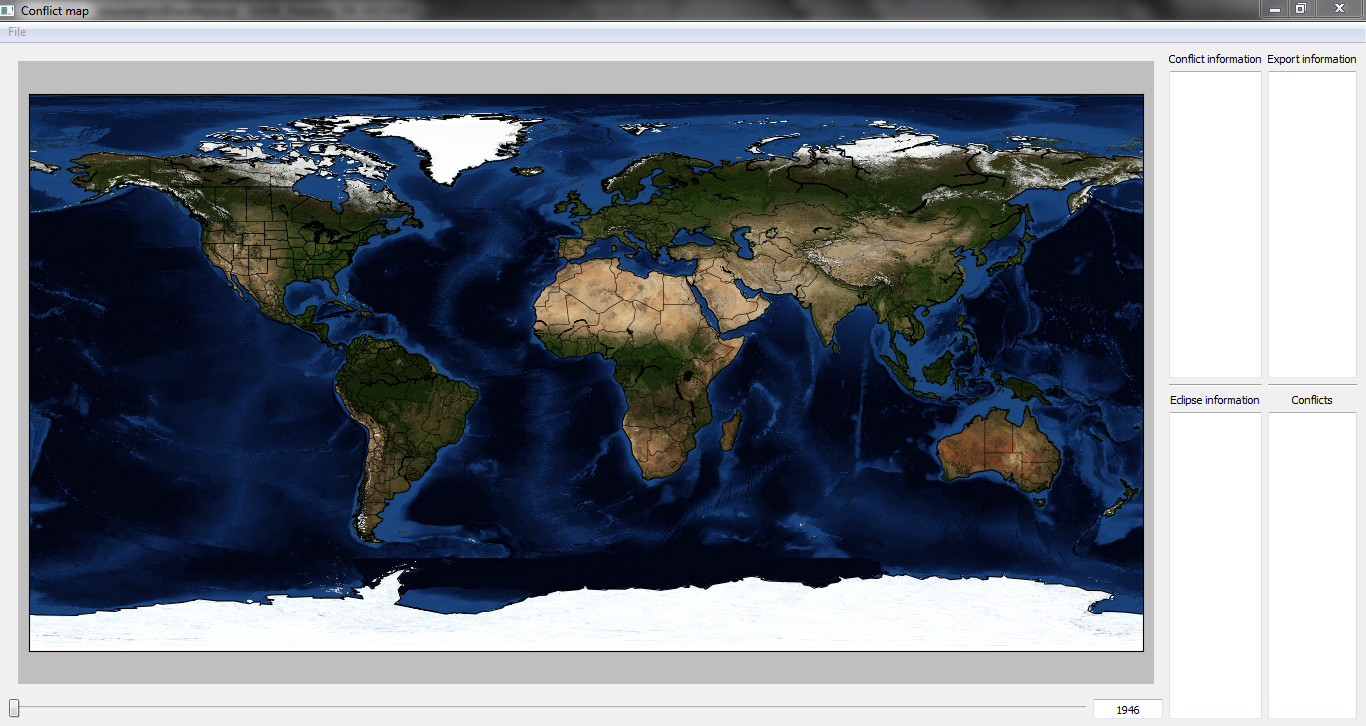
\includegraphics[width = 8cm]{openScreen.png}
		\caption*{Skjáviðmót á forriti}
	\end{figure}
\end{frame}

	
\begin{frame}
	\centering
	Þökkum góða áheyrn. \\
	Spurningar?\\
\end{frame}

\bibframe
\end{document}

%%% Local Variables:
%%% mode: latex
%%% TeX-master: t
%%% End:
